%% If you have any problems using this template, please contact the author: %%
%% Chris Carmona: carmona@stats.ox.ac.uk ; chriscarmona.me %%

\documentclass[aspectratio=169]{beamer}

\usepackage[UKenglish]{babel}
\usepackage[utf8]{inputenc} % so we can input characters with accents (e.g. ő)
\usepackage[export]{adjustbox}

%\usepackage{Presentation/Presentation_layout}
\usepackage{tikz}
\usetikzlibrary{calc,arrows,fadings, automata, positioning}
\tikzfading[name=fade inside,inner color=red,outer color=blue]
\usepackage{graphicx} % ease graphics management
\usepackage{xcolor}
\usepackage{minted}
\definecolor{codebgcolor}{rgb}{1,1,0.9}
\usemintedstyle{colorful}

\usefonttheme[onlymath]{serif}

%\usefonttheme{serif} % change font to allow \textbf{}
\usepackage{amsmath,amsthm,amssymb,mathtools} % for math equations
\usepackage[square,sort,comma,numbers]{natbib} % richer citation
\usepackage{breakcites} % avoid overfull hbox for long cites
\definecolor{kthBlue}{RGB}{25, 84, 166}          % Oxford Blue
\definecolor{bggrey}{RGB}{240, 240, 240}          % Oxford Blue

\usepackage{bm}

\usecolortheme{beaver}
\setbeamercolor{frametitle}{fg=white,bg=kthBlue}
\setbeamercolor{title}{fg=white,bg=kthBlue}
\setbeamercolor{section in toc}{fg=kthBlue}
\setbeamercolor{background canvas}{bg=bggrey}


\DeclareMathOperator{\newdiff}{d} % use \dif instead
\newcommand{\dif}{\newdiff\!}
\newcommand{\fdif}[2]{\dfrac{\dif #1}{\dif #2}}
\newcommand{\ffdif}[2]{\dfrac{\dif^2 #1}{\dif #2^2}}
\newcommand{\fndif}[3]{\dfrac{\dif^{#3} #1}{\dif #2^{#3}}}

\newcommand{\fpart}[2]{\dfrac{\partial #1}{\partial #2}}
\newcommand{\ffpart}[2]{\dfrac{\partial^2 #1}{\partial #2^2}}
\newcommand{\fnpart}[3]{\dfrac{\partial^{#3} #1}{\partial #2^{#3}}}

\newcommand{\bigoh}{\mathcal{O}}
\newcommand{\nth}[1]{\ensuremath{#1^\text{th}}}

\DeclarePairedDelimiter\abs{\lvert}{\rvert}%
\makeatletter
\let\oldabs\abs
\def\abs{\@ifstar{\oldabs}{\oldabs*}}
\newcommand\norm[1]{\left\lVert#1\right\rVert}

%% Information (author, title, etc.) %%


\title[Short Title]{% short title for footer
    \color{white} Final project
    \vspace{0.5cm}
}

\author{Miguel De Le Court}

\institute{
        \textit{Methods in High performance computing}\\
        \textit{DD2356}
        \vspace{0.5cm}
}
\date[Venue and Date]{% short date for footer
   Stockholm, June 2021 
}

%% Content of slides %%
%%%%%%%%%%%%%%%%%%%%
\begin{document}
%%%%%%%%%%%%%%%%%%%%

% Title slide %
{
    \setbeamertemplate{footline}{}
    \setbeamertemplate{headline}{}
    \setbeamercolor{background canvas}{bg = kthBlue}
    \setbeamercolor{normal text}{fg=white}
    \usebeamercolor[fg]{normal text}
    \maketitle
}

%----------------------------%
% Contents slide
%\setbeamertemplate{background canvas}{\begin{tikzpicture} \node[opacity=.1]{\includegraphics[width=\paperwidth]{Figures/Presentation/KTH_camp.png}};\end{tikzpicture}}
% only for the image:
% Conclusions
\begin{frame}{Outline}
\tableofcontents

\vfill
\begin{center}
    \footnotesize The last version of these slides and the code presented here are available at \url{https://github.com/MiguelDLC/DD2356-Project}    
\end{center}

\end{frame}
%----------------------------%

%now include the slides
\setbeamercovered{transparent}
%----------------------------%



% Introduction
%----------------------------%

\begin{frame}{Structure of the code}
    \inputminted[tabsize=4,fontsize=\scriptsize,framesep=2mm,bgcolor=codebgcolor,breaklines,linenos]{c}{../core.c}    
\end{frame}
%----------------------------%
\section{Structure of the code}
\begin{frame}{Structure of the code}
    \vspace{-0.8cm}
    \begin{figure}
        \centering
        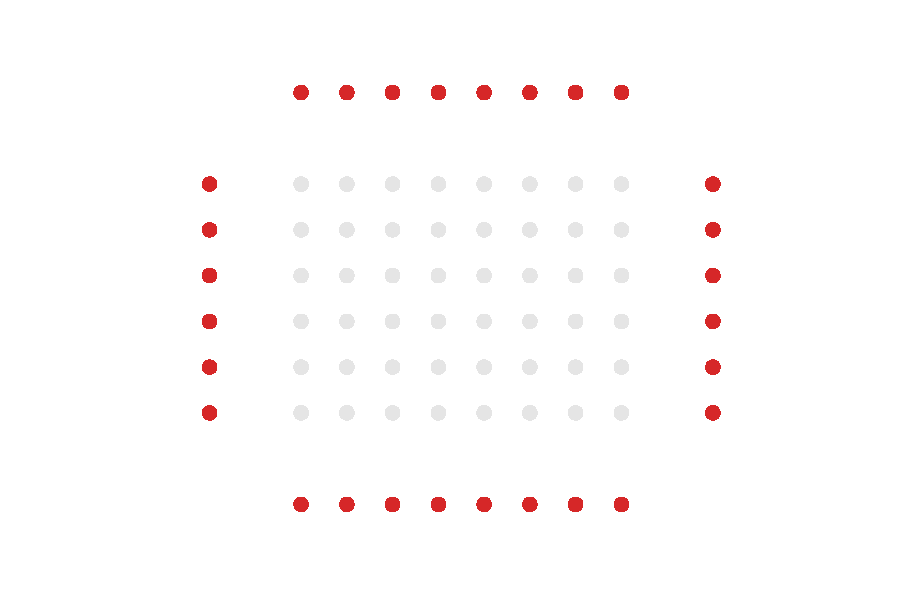
\includegraphics[width=0.8\linewidth]{Figures/step0.pdf}
    \end{figure}
    \vspace{-1.2cm}
    \inputminted[firstline=2, lastline=2,tabsize=4,fontsize=\footnotesize,framesep=2mm,bgcolor=codebgcolor,breaklines,linenos]{c}{../core.c}
\end{frame}

%----------------------------%

\begin{frame}{Structure of the code}
    \vspace{-0.8cm}
    \begin{figure}
        \centering
        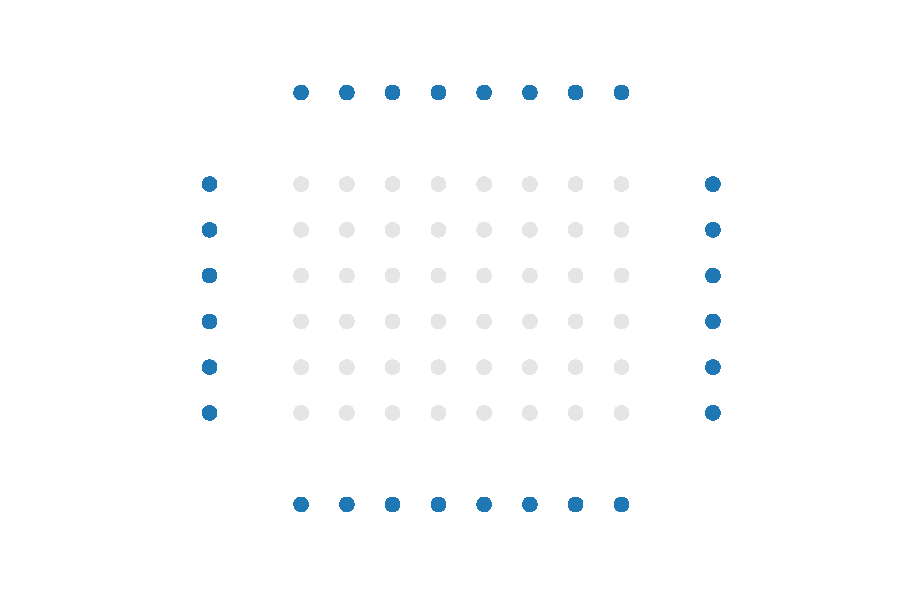
\includegraphics[width=0.8\linewidth]{Figures/step1.pdf}
    \end{figure}
    \vspace{-1.2cm}
    \inputminted[firstline=3, lastline=3,tabsize=4,fontsize=\footnotesize,framesep=2mm,bgcolor=codebgcolor,breaklines,linenos]{c}{../core.c}
\end{frame}

%----------------------------%

\begin{frame}{Structure of the code}
    \vspace{-0.8cm}
    \begin{figure}
        \centering
        
\includegraphics[width=0.8\linewidth]{Figures/step2.pdf}
    \end{figure}
    \vspace{-1.2cm}
    \inputminted[firstline=6, lastline=7,tabsize=4,fontsize=\footnotesize,framesep=2mm,bgcolor=codebgcolor,breaklines,linenos]{c}{../core.c}
\end{frame}

%----------------------------%

\begin{frame}{Structure of the code}
    \vspace{-0.8cm}
    \begin{figure}
        \centering
        
\includegraphics[width=0.8\linewidth]{Figures/step3.pdf}
    \end{figure}
    \vspace{-1.2cm}
    \inputminted[firstline=9, lastline=9,tabsize=4,fontsize=\footnotesize,framesep=2mm,bgcolor=codebgcolor,breaklines,linenos]{c}{../core.c}
\end{frame}

%----------------------------%


\begin{frame}{Structure of the code}
    \vspace{-0.8cm}
    \begin{figure}
        \centering
        
\includegraphics[width=0.8\linewidth]{Figures/step4.pdf}
    \end{figure}
    \vspace{-1.2cm}
    \inputminted[firstline=11, lastline=11,tabsize=4,fontsize=\footnotesize,framesep=2mm,bgcolor=codebgcolor,breaklines,linenos]{c}{../core.c}
\end{frame}

%----------------------------%


\section{Validation}
\subsection{Reference implementation}
\begin{frame}{Validation}
    Result computed with the MPI solver
    \begin{figure}
        \centering
        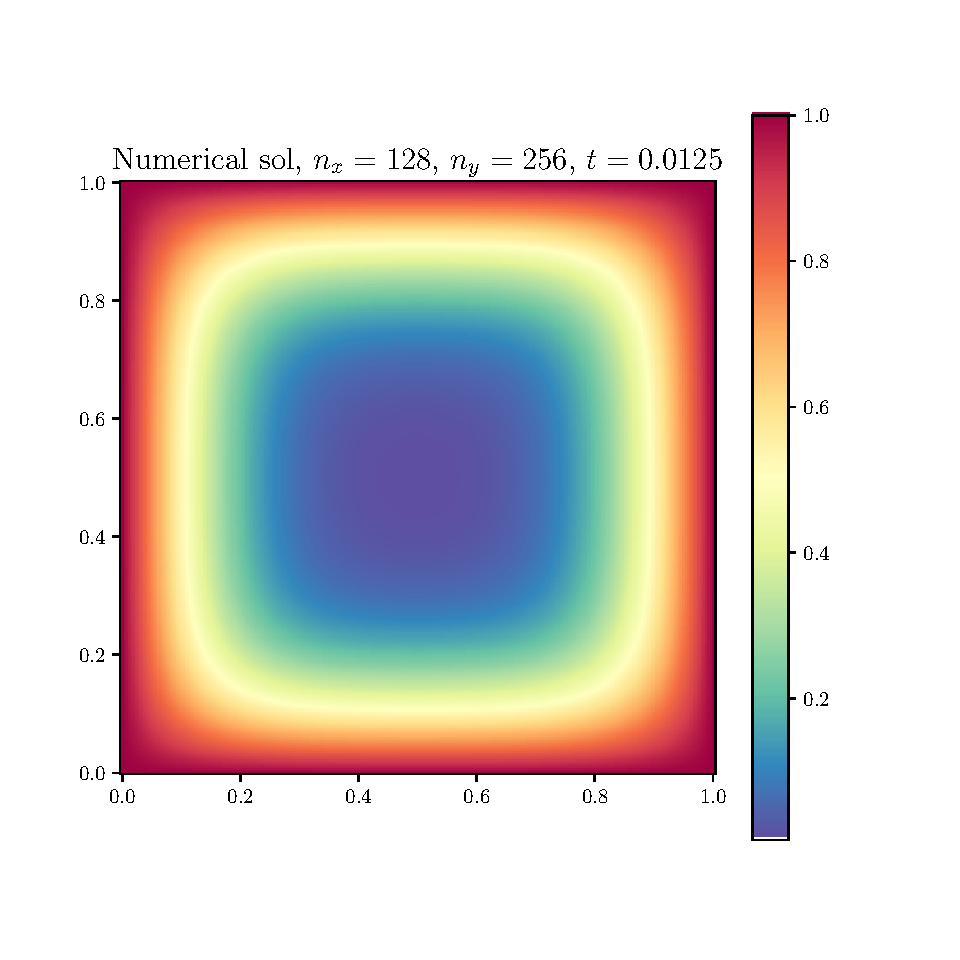
\includegraphics[height=8cm]{Figures/sol.pdf}
    \end{figure}
\end{frame}

%----------------------------%

\begin{frame}{Validation}
    \framesubtitle{Comparison with a reference implementation}
    First validation test : check against a reference implementation
    \begin{figure}
        \centering
        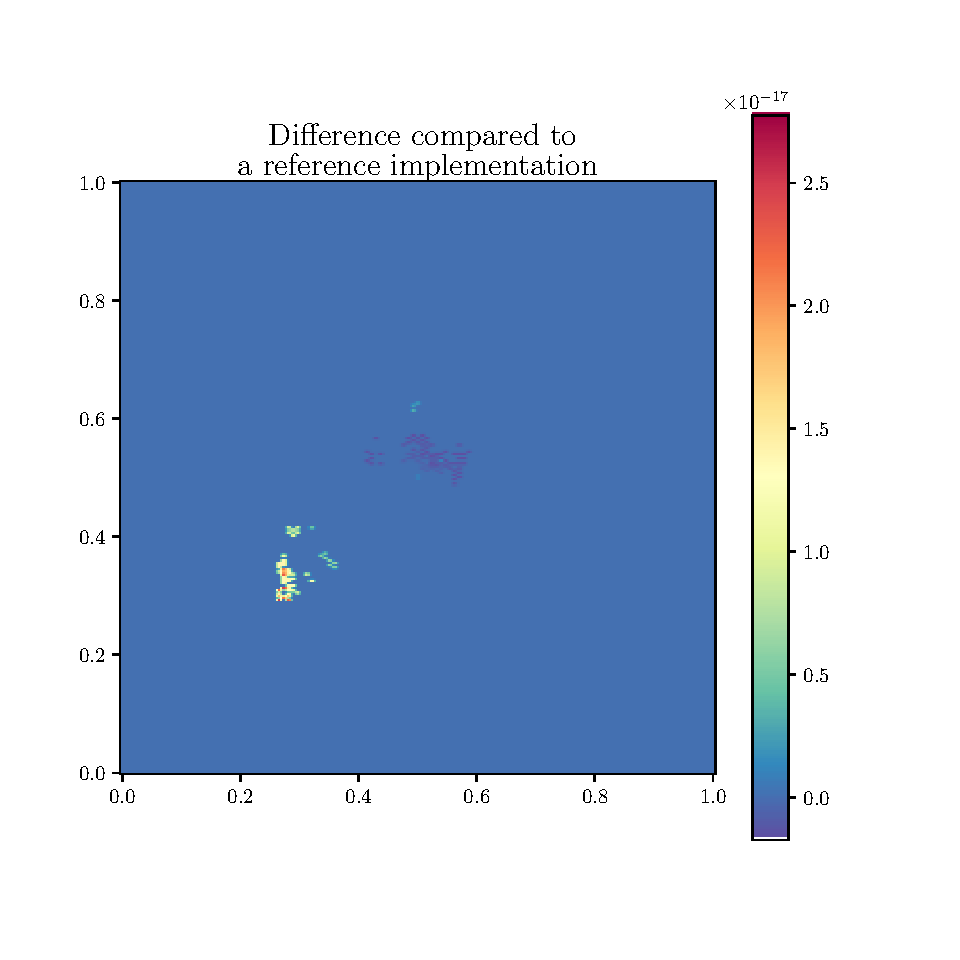
\includegraphics[height=8cm]{Figures/solcomp.pdf}
    \end{figure}
\end{frame}

%----------------------------%

\subsection{Comparison with the analytical solution}

\begin{frame}{Validation}
    \framesubtitle{Comparison with an analytical solution}
    Second validation test : check against a reference implementation and ensure that the error decreases as expected

    \vfill
    Expected error :
    \[
        \norm{\bm{T-T_\text{ref}}} = \bigoh(\Delta x^2) + \bigoh(\Delta t) = \bigoh(\Delta x^2)
    \]

    \vfill
    Analytical solution :
    \[
        T_\text{ref}(x, y, t) = 1- \dfrac{16}{\pi^2} \sum_{k \text{ odd}} \sum_{l \text{ odd}} \sin(k \pi x) \sin(l \pi y) e^{-\pi^2(k^2 + l^2) t}
    \]
    
\end{frame}

%----------------------------%

\begin{frame}{Validation}
    \framesubtitle{Comparison with an analytical solution}
    \begin{figure}
        \centering
        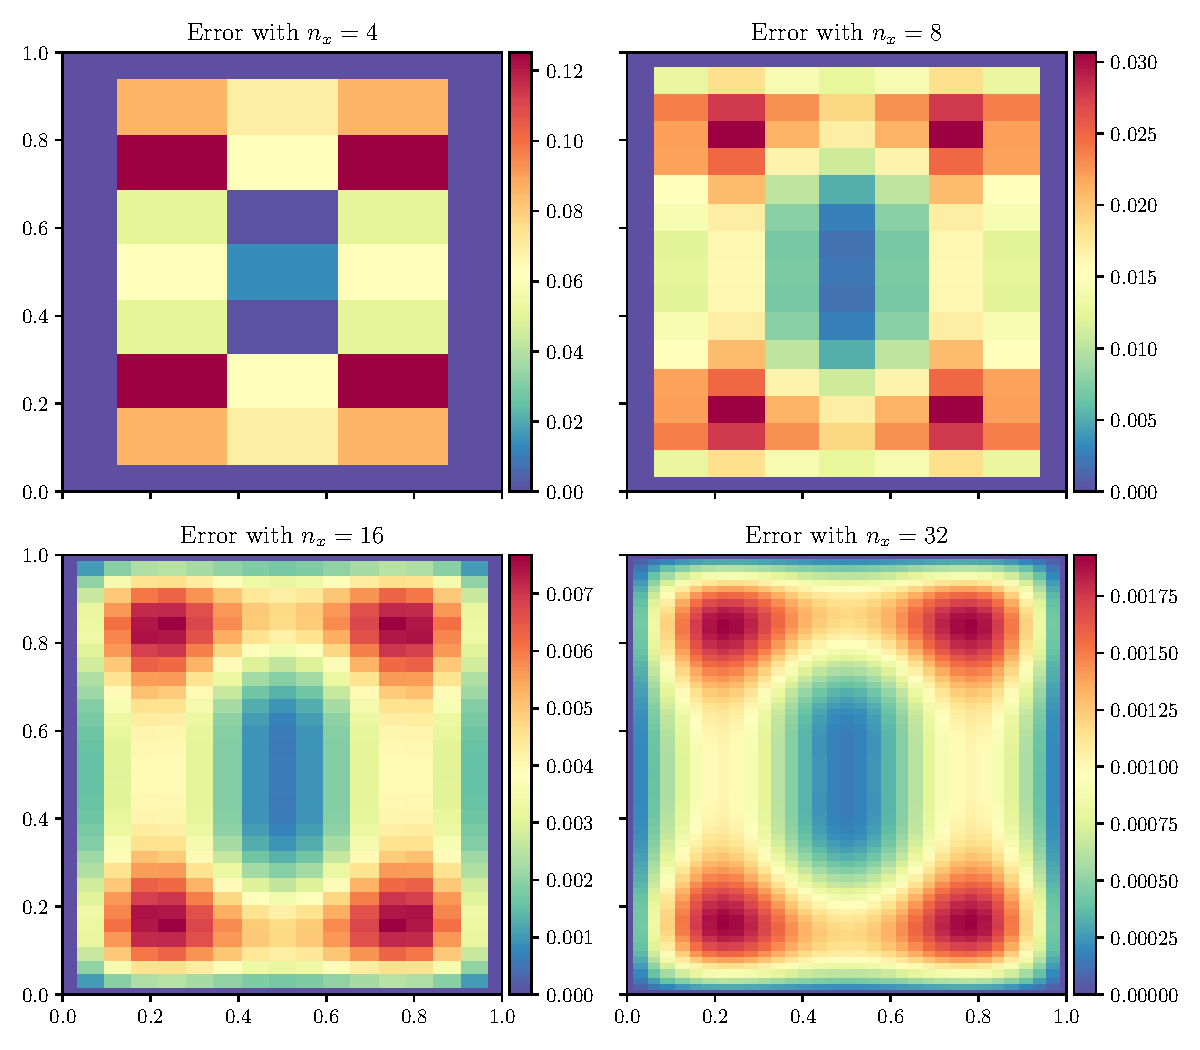
\includegraphics[height=7cm]{Figures/plotconverge.pdf}
    \end{figure}
\end{frame}

%----------------------------%

\begin{frame}{Validation}
    \framesubtitle{Comparison with an analytical solution}
    Second validation test : check against a reference implementation and ensure that the error decreases as expected

    \begin{figure}
        \centering
        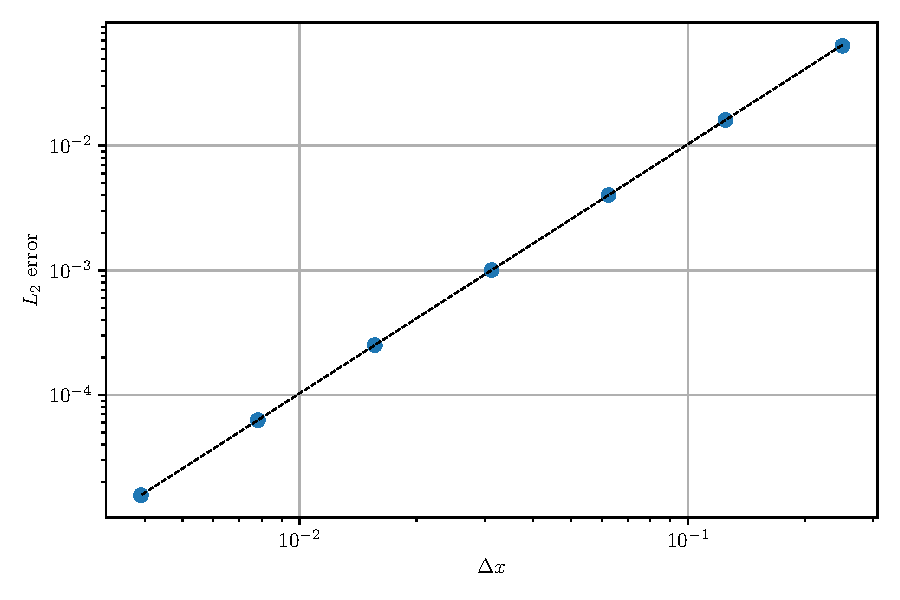
\includegraphics[width=0.6\linewidth]{Figures/Convergence.pdf}
    \end{figure}
\end{frame}

%----------------------------%

\section{Scaling}
\begin{frame}{Scaling}
    \begin{figure}
        \centering
        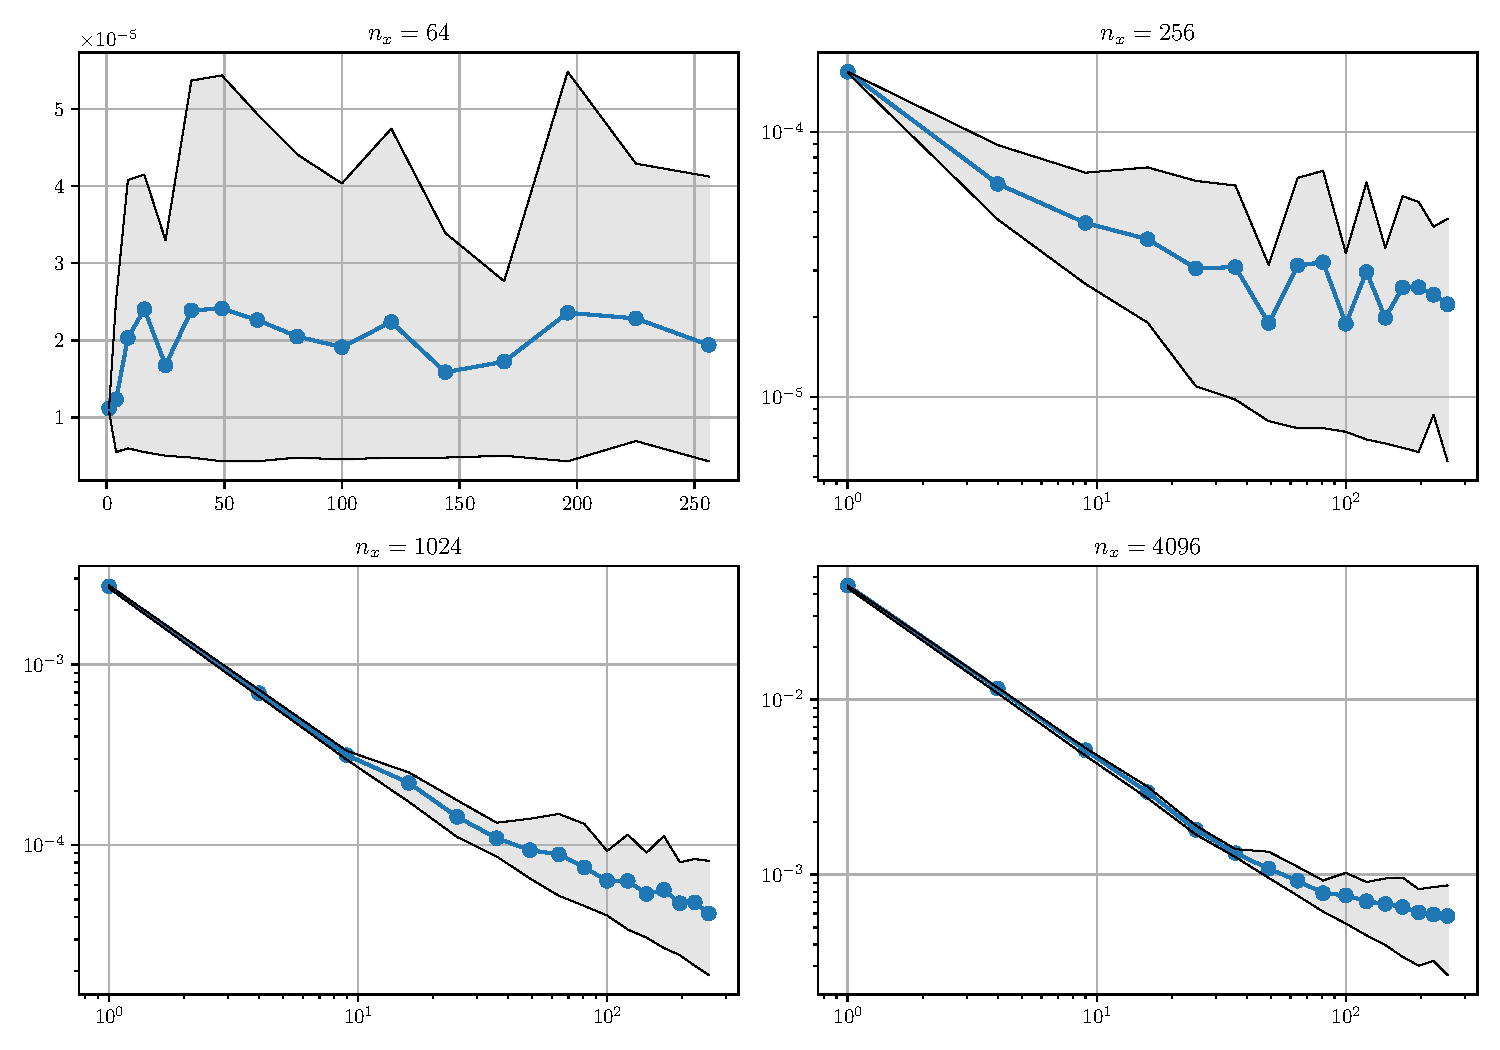
\includegraphics[width=0.75\linewidth]{Figures/strong_scaling.pdf}
    \end{figure}
\end{frame}

%----------------------------%

\section{Idle propagation}
\begin{frame}{Idle propagation}
    \inputminted[tabsize=4,fontsize=\scriptsize,framesep=2mm,bgcolor=codebgcolor,breaklines,linenos]{c}{../core2.c}    
\end{frame}

\begin{frame}{Idle propagation}
    \framesubtitle{Comparison with an analytical solution}
    \begin{figure}
        \centering
        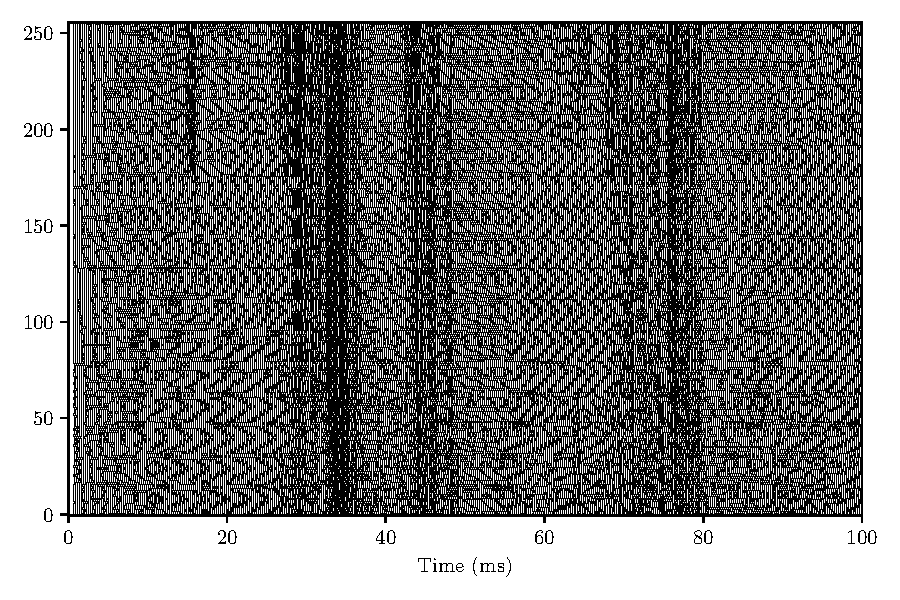
\includegraphics[width=0.8\linewidth]{Figures/idle_propagation.pdf}
    \end{figure}
\end{frame}

%----------------------------%

\begin{frame}{Idle propagation}
    \framesubtitle{Comparison with an analytical solution}
    \begin{figure}
        \centering
        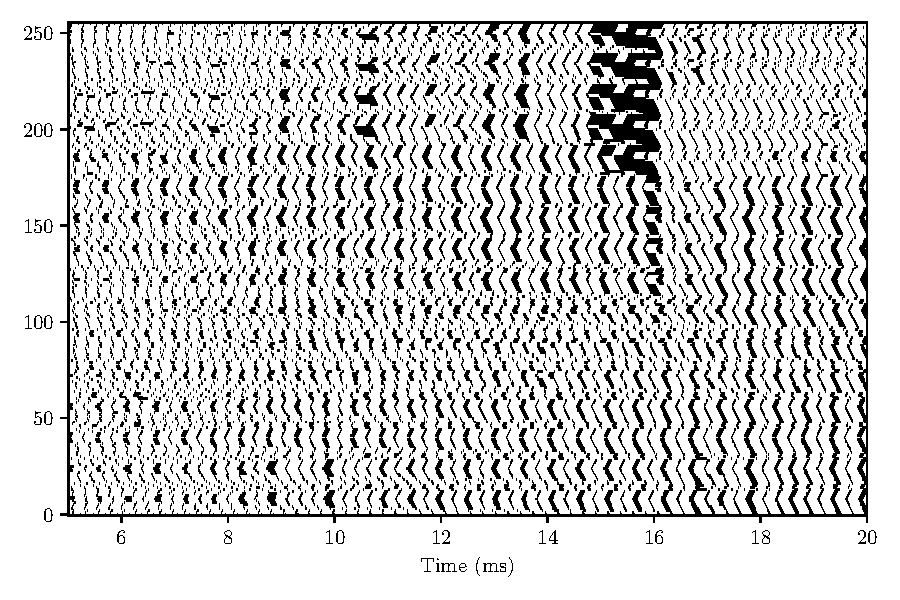
\includegraphics[width=0.8\linewidth]{Figures/idle_propagation_small.pdf}
    \end{figure}
\end{frame}

%%%%%%%%%%%%%%%%%%%%
\end{document}
%%%%%%%%%%%%%%%%%%%%
